\documentclass[11pt]{article}
\usepackage[margin=1in]{geometry}
\usepackage{amsmath,amssymb,booktabs,array,longtable}
\usepackage{graphicx}
\graphicspath{{figures/}}
\usepackage{hyperref}
\usepackage{enumitem}
\usepackage{titlesec}
\usepackage{float}
\usepackage{caption}
\usepackage{mathtools}
\usepackage{setspace}

\onehalfspacing

\begin{document}

\begin{center}
{\LARGE\textbf{Shiv Nadar University Chennai}}\\[4mm]
\end{center}

\renewcommand{\arraystretch}{1.6}
\setlength{\tabcolsep}{10pt}

\begin{center}
\begin{tabular}{|p{4cm}|p{9.5cm}|}
\hline
\textbf{Degree \& Branch} & B.Tech Artificial Intelligence \& Data Science, Semester V \\ \hline
\textbf{Subject} & CS3807 -- Deep Learning Laboratory \\ \hline
\textbf{Name} & Madhav.S \\ \hline
\textbf{Section} & AIDS `B' \\ \hline
\textbf{Register Number} & 24011101066 \\ \hline
\end{tabular}
\end{center}

\vspace{5mm}

\begin{center}
{\Large\textbf{Experiment 3}}\\[1mm]
{\large\textbf{Implementation of Convolutional Neural Networks (CNNs) for Image Classification}}
\end{center}

\vspace{4mm}

%----------------------------------------------------------

\section*{1. Objective}

To understand the working principle of Convolutional Neural Networks by implementing convolution, pooling, feature map visualization, and image classification using TensorFlow/Keras.

%----------------------------------------------------------

\section*{2. Learning Outcomes}

Students will be able to

\begin{enumerate}[leftmargin=*]
\item Explain the convolution operation.
\item Compute output dimensions using stride and padding.
\item Visualize feature maps.
\item Implement max pooling and average pooling.
\item Calculate CNN parameters.
\item Build a CNN for image classification.
\item Evaluate CNN performance.
\end{enumerate}

%----------------------------------------------------------

\section*{3. Background Theory}

A Convolutional Neural Network consists of

\begin{itemize}[leftmargin=*]
\item Convolution Layer
\item Activation Layer
\item Pooling Layer
\item Fully Connected Layer
\end{itemize}

The convolution operation is

\[
Y(i,j)=\sum_m\sum_n X(i+m,j+n)K(m,n)
\]

where

\begin{itemize}[leftmargin=*]
\item $X$ : Input Image
\item $K$ : Kernel (Filter)
\item $Y$ : Feature Map
\end{itemize}

The output feature map size is

\[
\frac{N-F+2P}{S}+1
\]

where

\begin{tabular}{ll}
$N$ & Input Size\\
$F$ & Filter Size\\
$P$ & Padding\\
$S$ & Stride
\end{tabular}

\subsection*{3.1 Common Convolution Kernels}

A \textbf{kernel} (or \textbf{filter}) is a small matrix that slides over an input image to extract important visual features such as edges, textures, corners, and smooth regions. During convolution, the kernel is multiplied element-wise with the corresponding image pixels, and the results are summed to produce a single value in the output feature map. Different kernels highlight different image characteristics.

\subsubsection*{Identity Kernel}
Preserves the original image without modifying its pixel values.
\[
\begin{bmatrix}
0 & 0 & 0\\
0 & 1 & 0\\
0 & 0 & 0
\end{bmatrix}
\]
\textbf{Purpose:} preserves the original image; used for understanding the convolution operation.

\subsubsection*{Sobel-X Kernel (Vertical Edge Detection)}
Detects vertical edges by measuring intensity changes along the horizontal direction.
\[
\begin{bmatrix}
-1 & 0 & 1\\
-2 & 0 & 2\\
-1 & 0 & 1
\end{bmatrix}
\]
\textbf{Applications:} object detection, lane detection, face recognition.

\subsubsection*{Sobel-Y Kernel (Horizontal Edge Detection)}
Detects horizontal edges by measuring intensity changes along the vertical direction.
\[
\begin{bmatrix}
-1 & -2 & -1\\
0 & 0 & 0\\
1 & 2 & 1
\end{bmatrix}
\]
\textbf{Applications:} text detection, boundary extraction, medical image analysis.

\subsubsection*{Laplacian Kernel}
Detects edges in all directions using the second-order derivative of image intensity.
\[
\begin{bmatrix}
0 & -1 & 0\\
-1 & 4 & -1\\
0 & -1 & 0
\end{bmatrix}
\]
\textbf{Applications:} edge enhancement, satellite image analysis, medical imaging.

\subsubsection*{Sharpening Kernel}
Enhances fine details by emphasizing high-frequency components.
\[
\begin{bmatrix}
0 & -1 & 0\\
-1 & 5 & -1\\
0 & -1 & 0
\end{bmatrix}
\]
\textbf{Applications:} image enhancement, OCR, face recognition.

\subsubsection*{Box Blur Kernel}
Smooths an image by replacing each pixel with the average of its neighboring pixels.
\[
\frac{1}{9}
\begin{bmatrix}
1 & 1 & 1\\
1 & 1 & 1\\
1 & 1 & 1
\end{bmatrix}
\]
\textbf{Applications:} noise removal, image smoothing, preprocessing.

\subsubsection*{Gaussian Blur Kernel}
Smooths the image while preserving overall structure better than a simple average filter.
\[
\frac{1}{16}
\begin{bmatrix}
1 & 2 & 1\\
2 & 4 & 2\\
1 & 2 & 1
\end{bmatrix}
\]
\textbf{Applications:} noise reduction, computer vision preprocessing, feature extraction.

\subsubsection*{Emboss Kernel}
Creates a three-dimensional appearance by emphasizing directional changes in intensity.
\[
\begin{bmatrix}
-2 & -1 & 0\\
-1 & 1 & 1\\
0 & 1 & 2
\end{bmatrix}
\]
\textbf{Applications:} texture analysis, artistic image effects.

\subsubsection*{Outline Detection Kernel}
Highlights object boundaries by emphasizing regions with rapid intensity changes.
\[
\begin{bmatrix}
-1 & -1 & -1\\
-1 & 8 & -1\\
-1 & -1 & -1
\end{bmatrix}
\]
\textbf{Applications:} image segmentation, boundary detection, shape extraction.

\subsubsection*{Motion Blur Kernel}
Simulates motion blur along the diagonal direction.
\[
\frac{1}{5}
\begin{bmatrix}
1 & 0 & 0 & 0 & 0\\
0 & 1 & 0 & 0 & 0\\
0 & 0 & 1 & 0 & 0\\
0 & 0 & 0 & 1 & 0\\
0 & 0 & 0 & 0 & 1
\end{bmatrix}
\]
\textbf{Applications:} motion simulation, image restoration, video processing.

\subsubsection*{Summary of Common Kernels}

\begin{center}
\renewcommand{\arraystretch}{1.3}
\begin{tabular}{|p{3cm}|p{2cm}|p{4cm}|p{4cm}|}
\hline
\textbf{Kernel} & \textbf{Size} & \textbf{Purpose} & \textbf{Applications}\\
\hline
Identity & $3\times3$ & Preserve original image & Baseline comparison\\
\hline
Sobel-X & $3\times3$ & Detect vertical edges & Object detection\\
\hline
Sobel-Y & $3\times3$ & Detect horizontal edges & Boundary detection\\
\hline
Laplacian & $3\times3$ & Detect edges in all directions & Medical imaging\\
\hline
Sharpen & $3\times3$ & Enhance details & Image enhancement\\
\hline
Box Blur & $3\times3$ & Smooth image & Noise removal\\
\hline
Gaussian Blur & $3\times3$ & Reduce noise & Computer vision\\
\hline
Emboss & $3\times3$ & 3D effect & Artistic filtering\\
\hline
Outline & $3\times3$ & Boundary extraction & Segmentation\\
\hline
Motion Blur & $5\times5$ & Simulate motion & Video processing\\
\hline
\end{tabular}
\end{center}

%----------------------------------------------------------

\section*{4. Numerical Example 1: Convolution}

Consider the following input image.
\[
X=
\begin{bmatrix}
1&2&3\\
4&5&6\\
7&8&9
\end{bmatrix}
\]
Kernel
\[
K=
\begin{bmatrix}
1&0\\
0&1
\end{bmatrix}
\]

First position: $1(1)+2(0)+4(0)+5(1)=6$\\
Second position: $2(1)+3(0)+5(0)+6(1)=8$\\
Third position: $4(1)+5(0)+7(0)+8(1)=12$\\
Fourth position: $5(1)+6(0)+8(0)+9(1)=14$

Feature Map
\[
\begin{bmatrix}
6&8\\
12&14
\end{bmatrix}
\]

%----------------------------------------------------------

\section*{5. Numerical Example 2: Max Pooling}

Feature map
\[
\begin{bmatrix}
1&5&2&3\\
7&8&1&0\\
4&6&9&5\\
2&3&1&8
\end{bmatrix}
\]

Using a $2\times2$ max pooling filter:

Window 1: $\begin{bmatrix}1&5\\7&8\end{bmatrix}\rightarrow 8$ \quad
Window 2: $\begin{bmatrix}2&3\\1&0\end{bmatrix}\rightarrow3$

Window 3: $\begin{bmatrix}4&6\\2&3\end{bmatrix}\rightarrow6$ \quad
Window 4: $\begin{bmatrix}9&5\\1&8\end{bmatrix}\rightarrow9$

Output
\[
\begin{bmatrix}
8&3\\
6&9
\end{bmatrix}
\]

%----------------------------------------------------------

\section*{6. Numerical Example 3: Parameter Calculation}

Suppose the input image is $32\times32\times3$, with a convolution layer of 16 filters, kernel size $3\times3$.
\[
\text{Parameters} = (3\times3\times3+1)\times16 = (27+1)\times16 = 448
\]
Therefore, total trainable parameters = 448.

%----------------------------------------------------------

\section*{7. Dataset}

\textbf{Dataset:} CIFAR-10

\begin{itemize}[leftmargin=*]
\item Training Images : 50,000
\item Testing Images : 10,000
\item Classes : 10
\item Image Size : $32\times32\times3$
\end{itemize}

All ten classes were confirmed exactly balanced at 5,000 images each in the training set (airplane, automobile, bird, cat, deer, dog, frog, horse, ship, truck), with no missing values.

%----------------------------------------------------------

\section*{8. Experimental Procedure}

\subsection*{Task 1 -- Dataset Loading}
CIFAR-10 was loaded via the Keras dataset API. Ten sample images were displayed, dataset dimensions were printed and verified (50,000 training / 10,000 test images, $32\times32\times3$), and the class distribution was plotted.

\subsection*{Task 2 -- Convolution Layer, Kernel Size Comparison}
A single convolution layer was applied to a sample image using three kernel sizes -- $3\times3$, $5\times5$, and $7\times7$ -- with `valid' padding and stride 1, recording the resulting feature map size for each.

\subsection*{Task 3 -- Stride and Padding}
The same sample image was convolved with stride 1 vs. stride 2, and with `same' vs. `valid' padding, computing the output dimensions for each combination directly from the formula in Section 3.

\subsection*{Task 4 -- Feature Map Visualization}
Intermediate activations were extracted from every convolutional layer of the trained CNN for a single test image, displaying 8 feature maps per layer.

\subsection*{Task 5 -- Pooling Comparison}
Max Pooling and Average Pooling were compared on both output size (identical for both, since pooling size/stride alone determines spatial shape) and classification accuracy (trained on identical smaller CNNs under matched conditions).

\subsection*{Task 6 -- CNN Construction and Training}
Per the manual's specification, a CNN with the architecture
\[
\text{Input} \rightarrow \text{Conv} \rightarrow \text{ReLU} \rightarrow \text{MaxPool} \rightarrow \text{Conv} \rightarrow \text{ReLU} \rightarrow \text{MaxPool} \rightarrow \text{Flatten} \rightarrow \text{Dense} \rightarrow \text{Softmax}
\]
was built and trained with the Adam optimizer, 20 epochs, batch size 32. \textit{Note: alongside this manual-specification model, a larger, more elaborate CNN (5 convolutional layers across 3 blocks, with batch normalization, dropout, data augmentation, and a learning-rate schedule) was also built and trained, and is used for the main evaluation, feature map visualization, and pooling/hyperparameter studies throughout this report. Both models' results are reported separately and labelled clearly below, since they answer different parts of the manual.}

\subsection*{Task 7 -- Evaluation}
Both models were evaluated using accuracy, precision, recall, F1-score, a full classification report, and a confusion matrix.

%----------------------------------------------------------

\section*{9. Source Code}

The complete implementation, exactly as run in Colab, is hosted on GitHub.

\begin{center}
\url{https://github.com/smadhav2024/Deep_Learning_Lab}
\end{center}

%----------------------------------------------------------

\section*{10. Results}

\subsection*{10.1 Main CNN -- Architecture and Parameters}

\begin{table}[H]
\centering
\caption{Trainable Parameters of Convolutional Layers (Main CNN)}
\begin{tabular}{lccc}
\toprule
Layer & Output Shape & Params \\
\midrule
conv1 & $(32,32,32)$ & 896 \\
conv2 & $(32,32,32)$ & 9{,}248 \\
conv3 & $(16,16,64)$ & 18{,}496 \\
conv4 & $(16,16,64)$ & 36{,}928 \\
conv5 & $(8,8,128)$ & 73{,}856 \\
\bottomrule
\end{tabular}
\end{table}

\textbf{Total Convolutional Layer Parameters:} 139,424 \quad \textbf{Total Model Parameters:} 668,842

A manual check for \texttt{conv1} confirms the formula from Section 6: $(3\times3\times3+1)\times32 = 896$, matching Keras's own count exactly.

\subsection*{10.2 Main CNN -- Training and Test Performance}

The model was trained for 30 epochs at an initial learning rate of 0.001, batch size 64, with data augmentation and \texttt{ReduceLROnPlateau} monitoring validation loss (factor 0.5, patience 3). The learning rate was reduced three times over training -- at epoch 14 ($0.001\rightarrow0.0005$), epoch 20 ($0.0005\rightarrow0.00025$), and epoch 25 ($0.00025\rightarrow0.000125$).

\begin{table}[H]
\centering
\caption{Main CNN -- Test Set Performance}
\begin{tabular}{lc}
\toprule
Metric & Value \\
\midrule
Test Loss & 0.5095 \\
Accuracy & 0.8257 \\
Precision (weighted) & 0.8341 \\
Recall (weighted) & 0.8257 \\
F1-score (weighted) & 0.8235 \\
\bottomrule
\end{tabular}
\end{table}

\begin{table}[H]
\centering
\caption{Per-Class Classification Report (Main CNN)}
\begin{tabular}{lccc}
\toprule
Class & Precision & Recall & F1-score \\
\midrule
airplane   & 0.83 & 0.87 & 0.85 \\
automobile & 0.91 & 0.95 & 0.93 \\
bird       & 0.86 & 0.69 & 0.77 \\
cat        & 0.78 & 0.61 & 0.68 \\
deer       & 0.79 & 0.82 & 0.80 \\
dog        & 0.85 & 0.66 & 0.75 \\
frog       & 0.65 & 0.96 & 0.78 \\
horse      & 0.88 & 0.85 & 0.87 \\
ship       & 0.92 & 0.92 & 0.92 \\
truck      & 0.87 & 0.92 & 0.89 \\
\bottomrule
\end{tabular}
\end{table}

Vehicle classes (automobile, ship, truck) all cross 0.89 F1, while \textbf{cat} is the weakest class by recall (0.61) and \textbf{frog} shows the opposite pattern -- very high recall (0.96) but the lowest precision of any class (0.65) -- suggesting the model over-predicts frog somewhat, likely absorbing some of the missed cats and dogs. This cat/dog/frog overlap is a well-known difficulty in CIFAR-10 at this resolution.

\subsection*{10.3 Manual-Specification CNN (Task 6) -- Performance}

\begin{table}[H]
\centering
\caption{Manual-Specification CNN -- Test Set Performance}
\begin{tabular}{lc}
\toprule
Metric & Value \\
\midrule
Test Loss & 1.4740 \\
Accuracy & 0.6587 \\
Precision (weighted) & 0.6701 \\
Recall (weighted) & 0.6587 \\
F1-score (weighted) & 0.6606 \\
Total Parameters & 60,362 \\
\bottomrule
\end{tabular}
\end{table}

\begin{table}[H]
\centering
\caption{Per-Class Classification Report (Manual-Specification CNN)}
\begin{tabular}{lccc}
\toprule
Class & Precision & Recall & F1-score \\
\midrule
airplane   & 0.65 & 0.77 & 0.71 \\
automobile & 0.84 & 0.73 & 0.78 \\
bird       & 0.59 & 0.48 & 0.53 \\
cat        & 0.46 & 0.51 & 0.48 \\
deer       & 0.61 & 0.60 & 0.61 \\
dog        & 0.50 & 0.62 & 0.55 \\
frog       & 0.83 & 0.64 & 0.72 \\
horse      & 0.70 & 0.72 & 0.71 \\
ship       & 0.73 & 0.82 & 0.77 \\
truck      & 0.78 & 0.70 & 0.74 \\
\bottomrule
\end{tabular}
\end{table}

The simpler two-conv-layer architecture lands about 17 points behind the main CNN (65.87\% vs. 82.57\%), which makes sense given it has no batch normalization, no dropout, and roughly a ninth of the parameters (60,362 vs. 668,842). Its training log also shows a telling pattern: training accuracy climbs to 87.5\% by epoch 20, while validation accuracy peaks around epoch 4 (68\%) and then slowly \textit{drops} to 67.8\% by the final epoch, even as training loss keeps falling -- a textbook overfitting signature, and exactly what the regularization techniques in the main CNN (Section 10.1) were added to prevent.

\subsection*{10.4 Task 2 -- Kernel Size Comparison}

\begin{table}[H]
\centering
\caption{Effect of Kernel Size on Output Feature Map Size (32×32 input, stride 1, `valid' padding)}
\begin{tabular}{lccc}
\toprule
Kernel Size & Formula & Output Shape \\
\midrule
$3\times3$ & $(32-3+0)/1+1$ & $30\times30$ \\
$5\times5$ & $(32-5+0)/1+1$ & $28\times28$ \\
$7\times7$ & $(32-7+0)/1+1$ & $26\times26$ \\
\bottomrule
\end{tabular}
\end{table}

\subsection*{10.5 Task 3 -- Stride and Padding}

\begin{table}[H]
\centering
\caption{Effect of Stride (kernel $3\times3$, `valid' padding)}
\begin{tabular}{lcc}
\toprule
Stride & Formula & Output Shape \\
\midrule
1 & $(32-3+0)/1+1$ & $30\times30$ \\
2 & $(32-3+0)/2+1$ & $15\times15$ \\
\bottomrule
\end{tabular}
\end{table}

\begin{table}[H]
\centering
\caption{Effect of Padding (kernel $3\times3$, stride 1)}
\begin{tabular}{lc}
\toprule
Padding & Output Shape \\
\midrule
Same & $32\times32$ \\
Valid & $30\times30$ \\
\bottomrule
\end{tabular}
\end{table}

\subsection*{10.6 Task 5 -- Pooling: Output Size and Accuracy}

Both Max Pooling and Average Pooling, applied to a $32\times32\times16$ feature map with a $2\times2$ pool, produce an identical $16\times16\times16$ output -- output size depends only on pool size and stride, not on which pooling operation is used.

\begin{table}[H]
\centering
\caption{Max Pooling vs. Average Pooling -- Test Accuracy (small CNN, 8 epochs)}
\begin{tabular}{lc}
\toprule
Pooling Type & Test Accuracy \\
\midrule
Max Pooling & 0.5567 \\
Average Pooling & 0.5432 \\
\bottomrule
\end{tabular}
\end{table}

Max Pooling comes out about 1.4 points ahead of Average Pooling under identical short-training conditions -- the output shapes are indistinguishable, but the values each window produces clearly aren't, and that difference is what shows up in accuracy.

%----------------------------------------------------------

\section*{11. Mandatory Plots}

\begin{figure}[H]
\centering

\includegraphics[width=0.6\textwidth]{class_distribution.pdf}
\caption{Class Distribution in the CIFAR-10 Training Set}
\end{figure}
\textbf{Inference:} All ten classes contain exactly 5,000 images, confirming the dataset is perfectly balanced -- no resampling or class weighting was needed before training.

\begin{figure}[H]
\centering

\includegraphics[width=0.85\textwidth]{sample_images.pdf}
\caption{Sample Images -- One per Class}
\end{figure}
\textbf{Inference:} Even at $32\times32$ resolution, most classes are visually distinguishable, though cat, dog, and deer share enough colour and pose overlap to foreshadow the confusion seen later in both classification reports.

\begin{figure}[H]
\centering
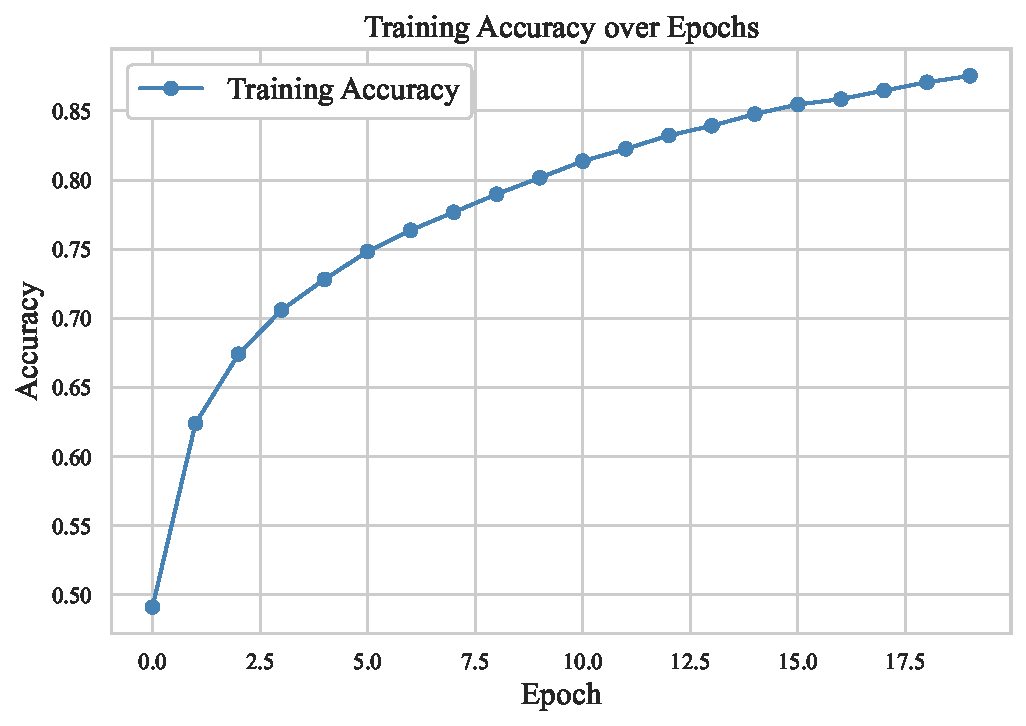
\includegraphics[width=0.7\textwidth]{training_accuracy.pdf}
\caption{Training Accuracy over Epochs (Manual-Specification CNN, Task 6)}
\end{figure}
\textbf{Inference:} Training accuracy climbs steadily and almost linearly, reaching 87.5\% by epoch 20 -- with no dropout or batch normalization holding it back, this simpler network fits the training set increasingly well, for better or worse.

\begin{figure}[H]
\centering
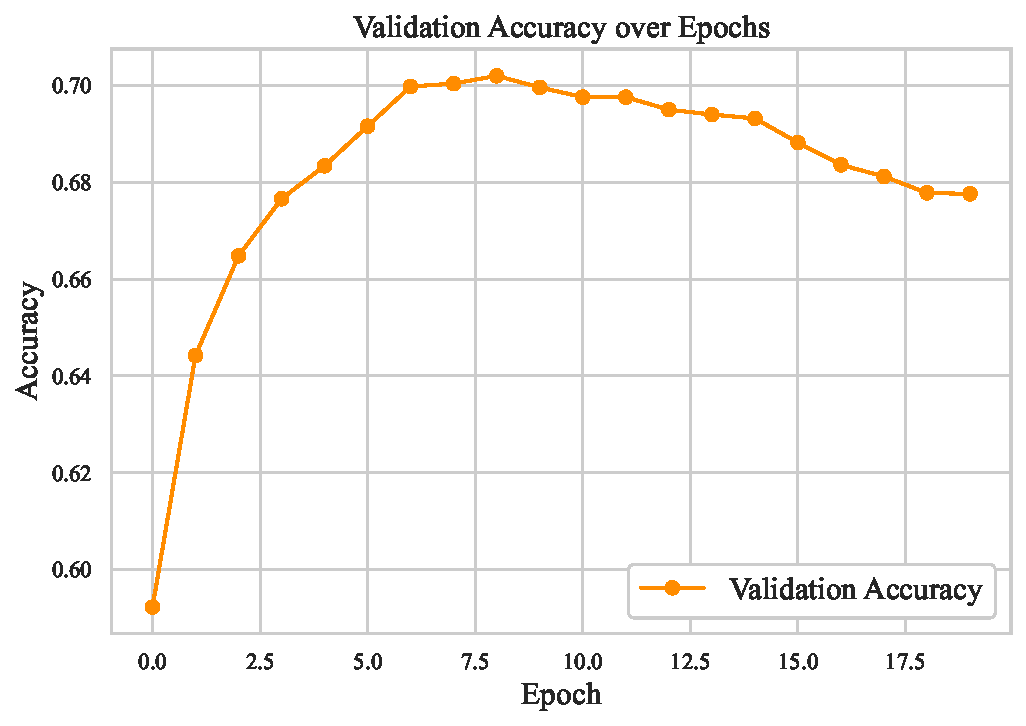
\includegraphics[width=0.7\textwidth]{validation_accuracy.pdf}
\caption{Validation Accuracy over Epochs (Manual-Specification CNN, Task 6)}
\end{figure}
\textbf{Inference:} Validation accuracy peaks early (around epoch 4, roughly 68\%) and then gradually declines to 67.8\% by epoch 20, even while training accuracy keeps rising -- the gap between these two curves is overfitting, made directly visible.

\begin{figure}[H]
\centering
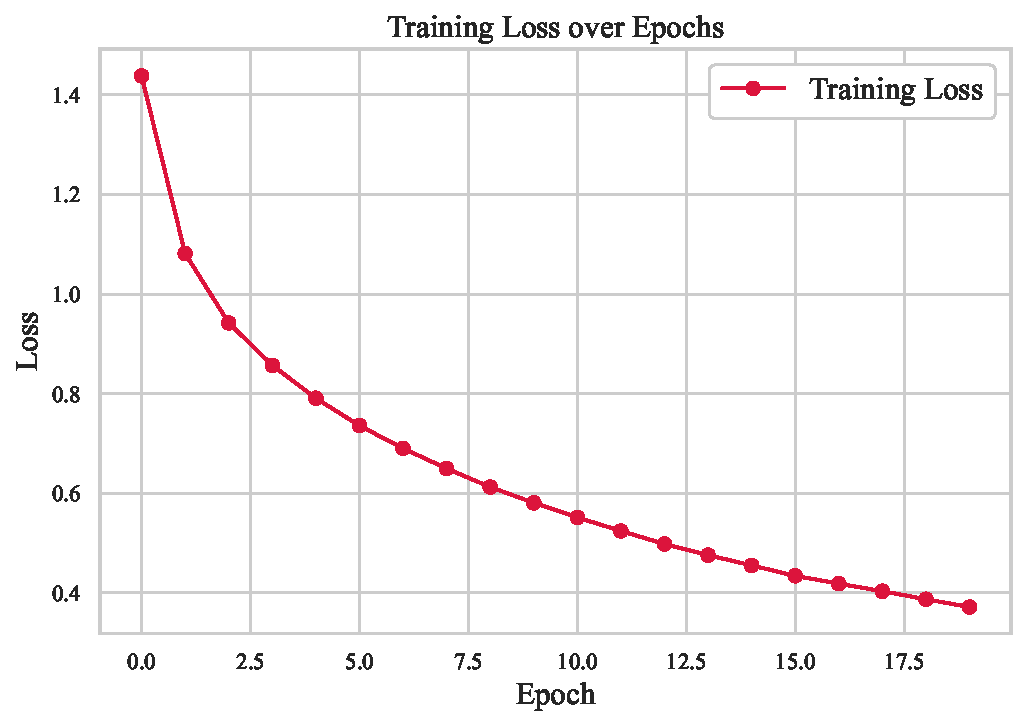
\includegraphics[width=0.7\textwidth]{training_loss.pdf}
\caption{Training Loss over Epochs (Manual-Specification CNN, Task 6)}
\end{figure}
\textbf{Inference:} Training loss falls smoothly and continuously across all 20 epochs (1.44 $\rightarrow$ 0.37), with no sign of plateauing -- the model keeps finding ways to fit the training data better, right up to the last epoch.

\begin{figure}[H]
\centering
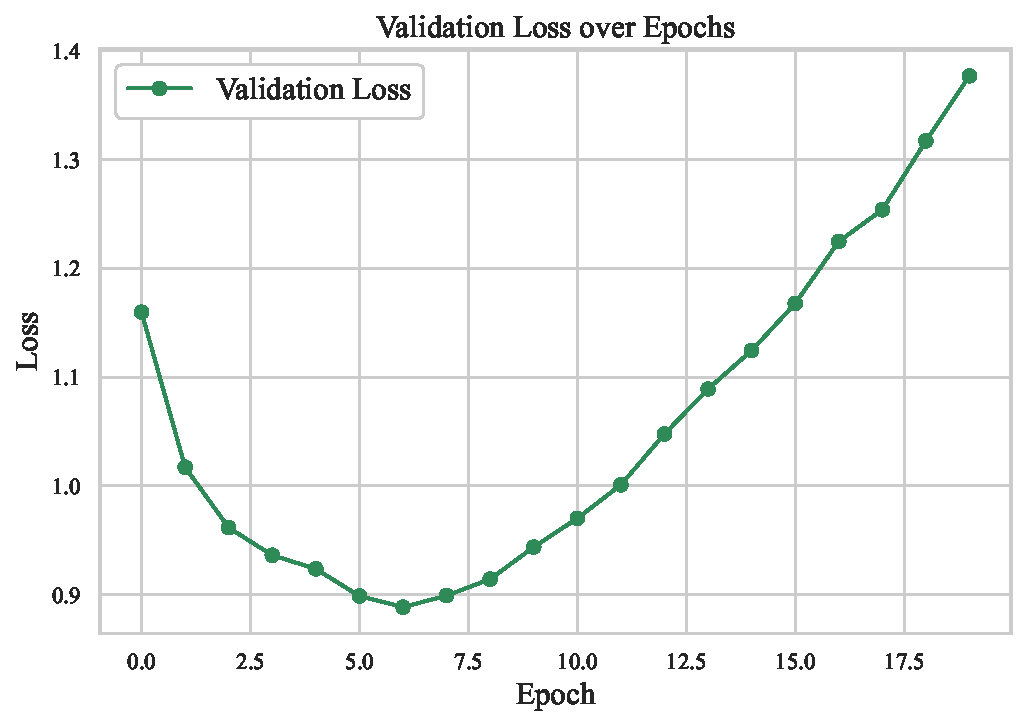
\includegraphics[width=0.7\textwidth]{validation_loss.pdf}
\caption{Validation Loss over Epochs (Manual-Specification CNN, Task 6)}
\end{figure}
\textbf{Inference:} Unlike training loss, validation loss bottoms out early (around epoch 3-4) and then climbs steadily for the rest of training, ending noticeably higher than where it started improving from -- since Task 6 doesn't call for early stopping, this rise is left fully visible, and it's the clearest single piece of evidence that this architecture overfits without regularization.

\begin{figure}[H]
\centering
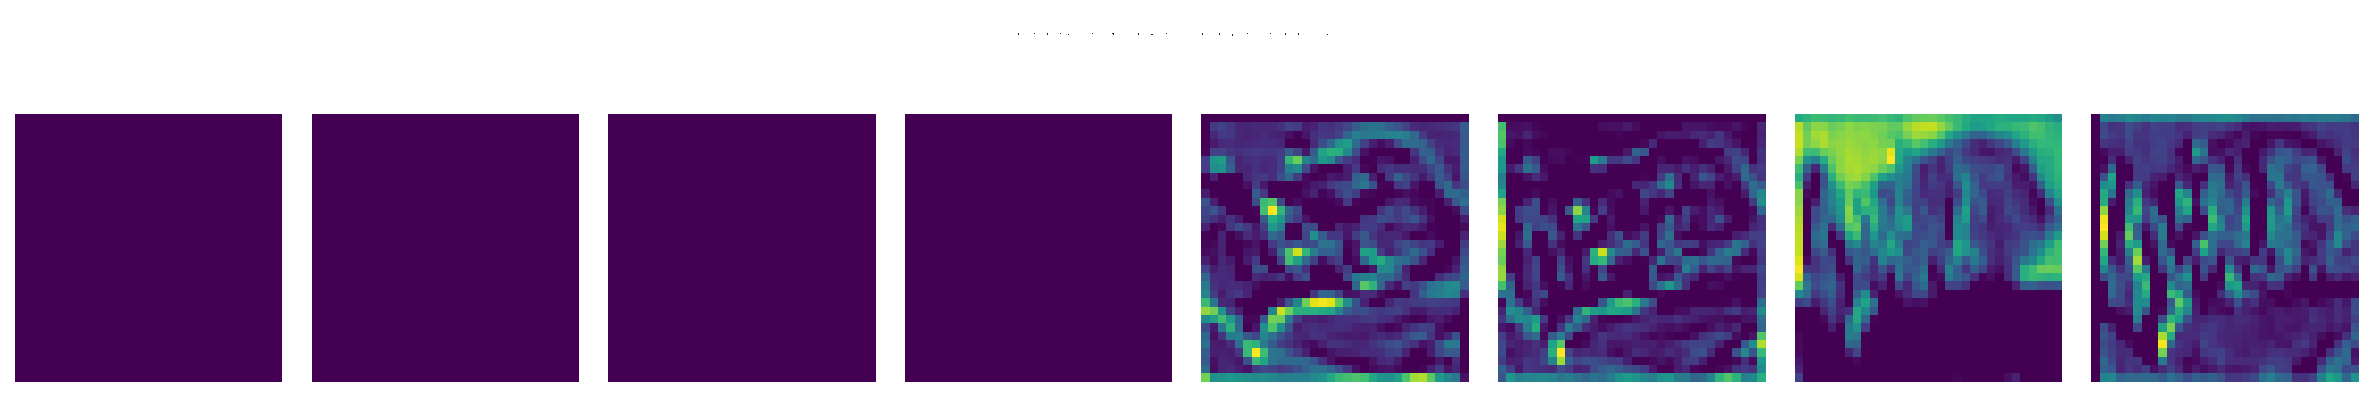
\includegraphics[width=\textwidth]{feature_maps_conv1.pdf}
\caption{Feature Maps -- Layer conv1 (Main CNN)}
\end{figure}
\textbf{Inference:} The earliest layer's feature maps closely resemble the input image, picking out simple edges and coarse shapes -- exactly what a first convolutional layer is expected to learn, and a direct visual match for the edge-detecting kernels discussed in Section 3.1.

\begin{figure}[H]
\centering

\includegraphics[width=0.6\textwidth]{confusion_matrix.pdf}
\caption{Confusion Matrix on the Test Set (Main CNN)}
\end{figure}
\textbf{Inference:} The diagonal clearly dominates, matching the 82.57\% overall accuracy, with visible off-diagonal mass sitting specifically around the cat/dog/bird block -- consistent with cat's low recall and frog's low precision in the classification report above.

%----------------------------------------------------------

\section*{12. Additional Generated Plots}

Beyond the eight mandatory plots, the following were also generated during this experiment.

\begin{figure}[H]
\centering
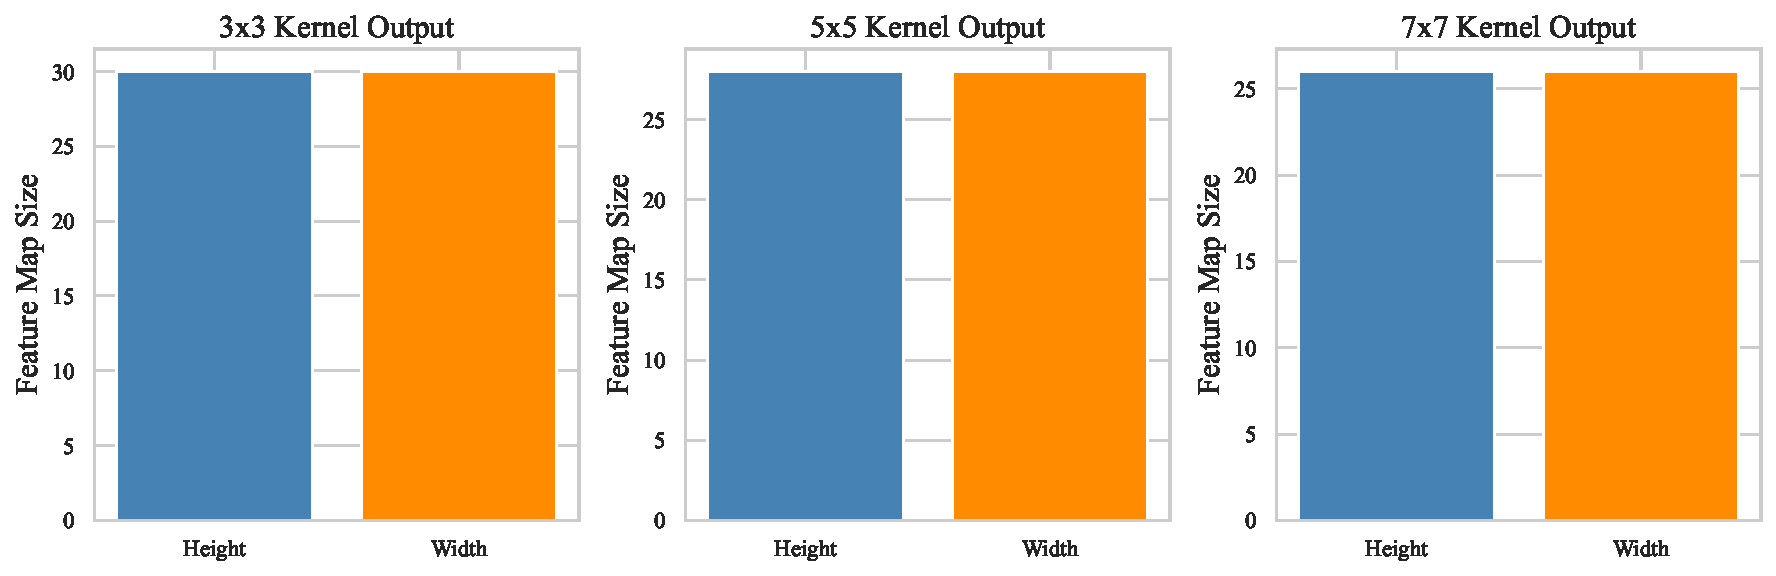
\includegraphics[width=0.9\textwidth]{kernel_size_comparison.pdf}
\caption{Output Feature Map Size for $3\times3$, $5\times5$, $7\times7$ Kernels}
\end{figure}
\textbf{Inference:} Larger kernels shrink the output feature map faster under `valid' padding -- a $7\times7$ kernel leaves a $26\times26$ output from a $32\times32$ input, while a $3\times3$ kernel only shrinks it to $30\times30$. This is exactly why every convolutional layer in the main CNN uses `same' padding instead -- stacking several `valid'-padded layers would shrink the feature map away almost entirely before reaching the classifier.

\begin{figure}[H]
\centering
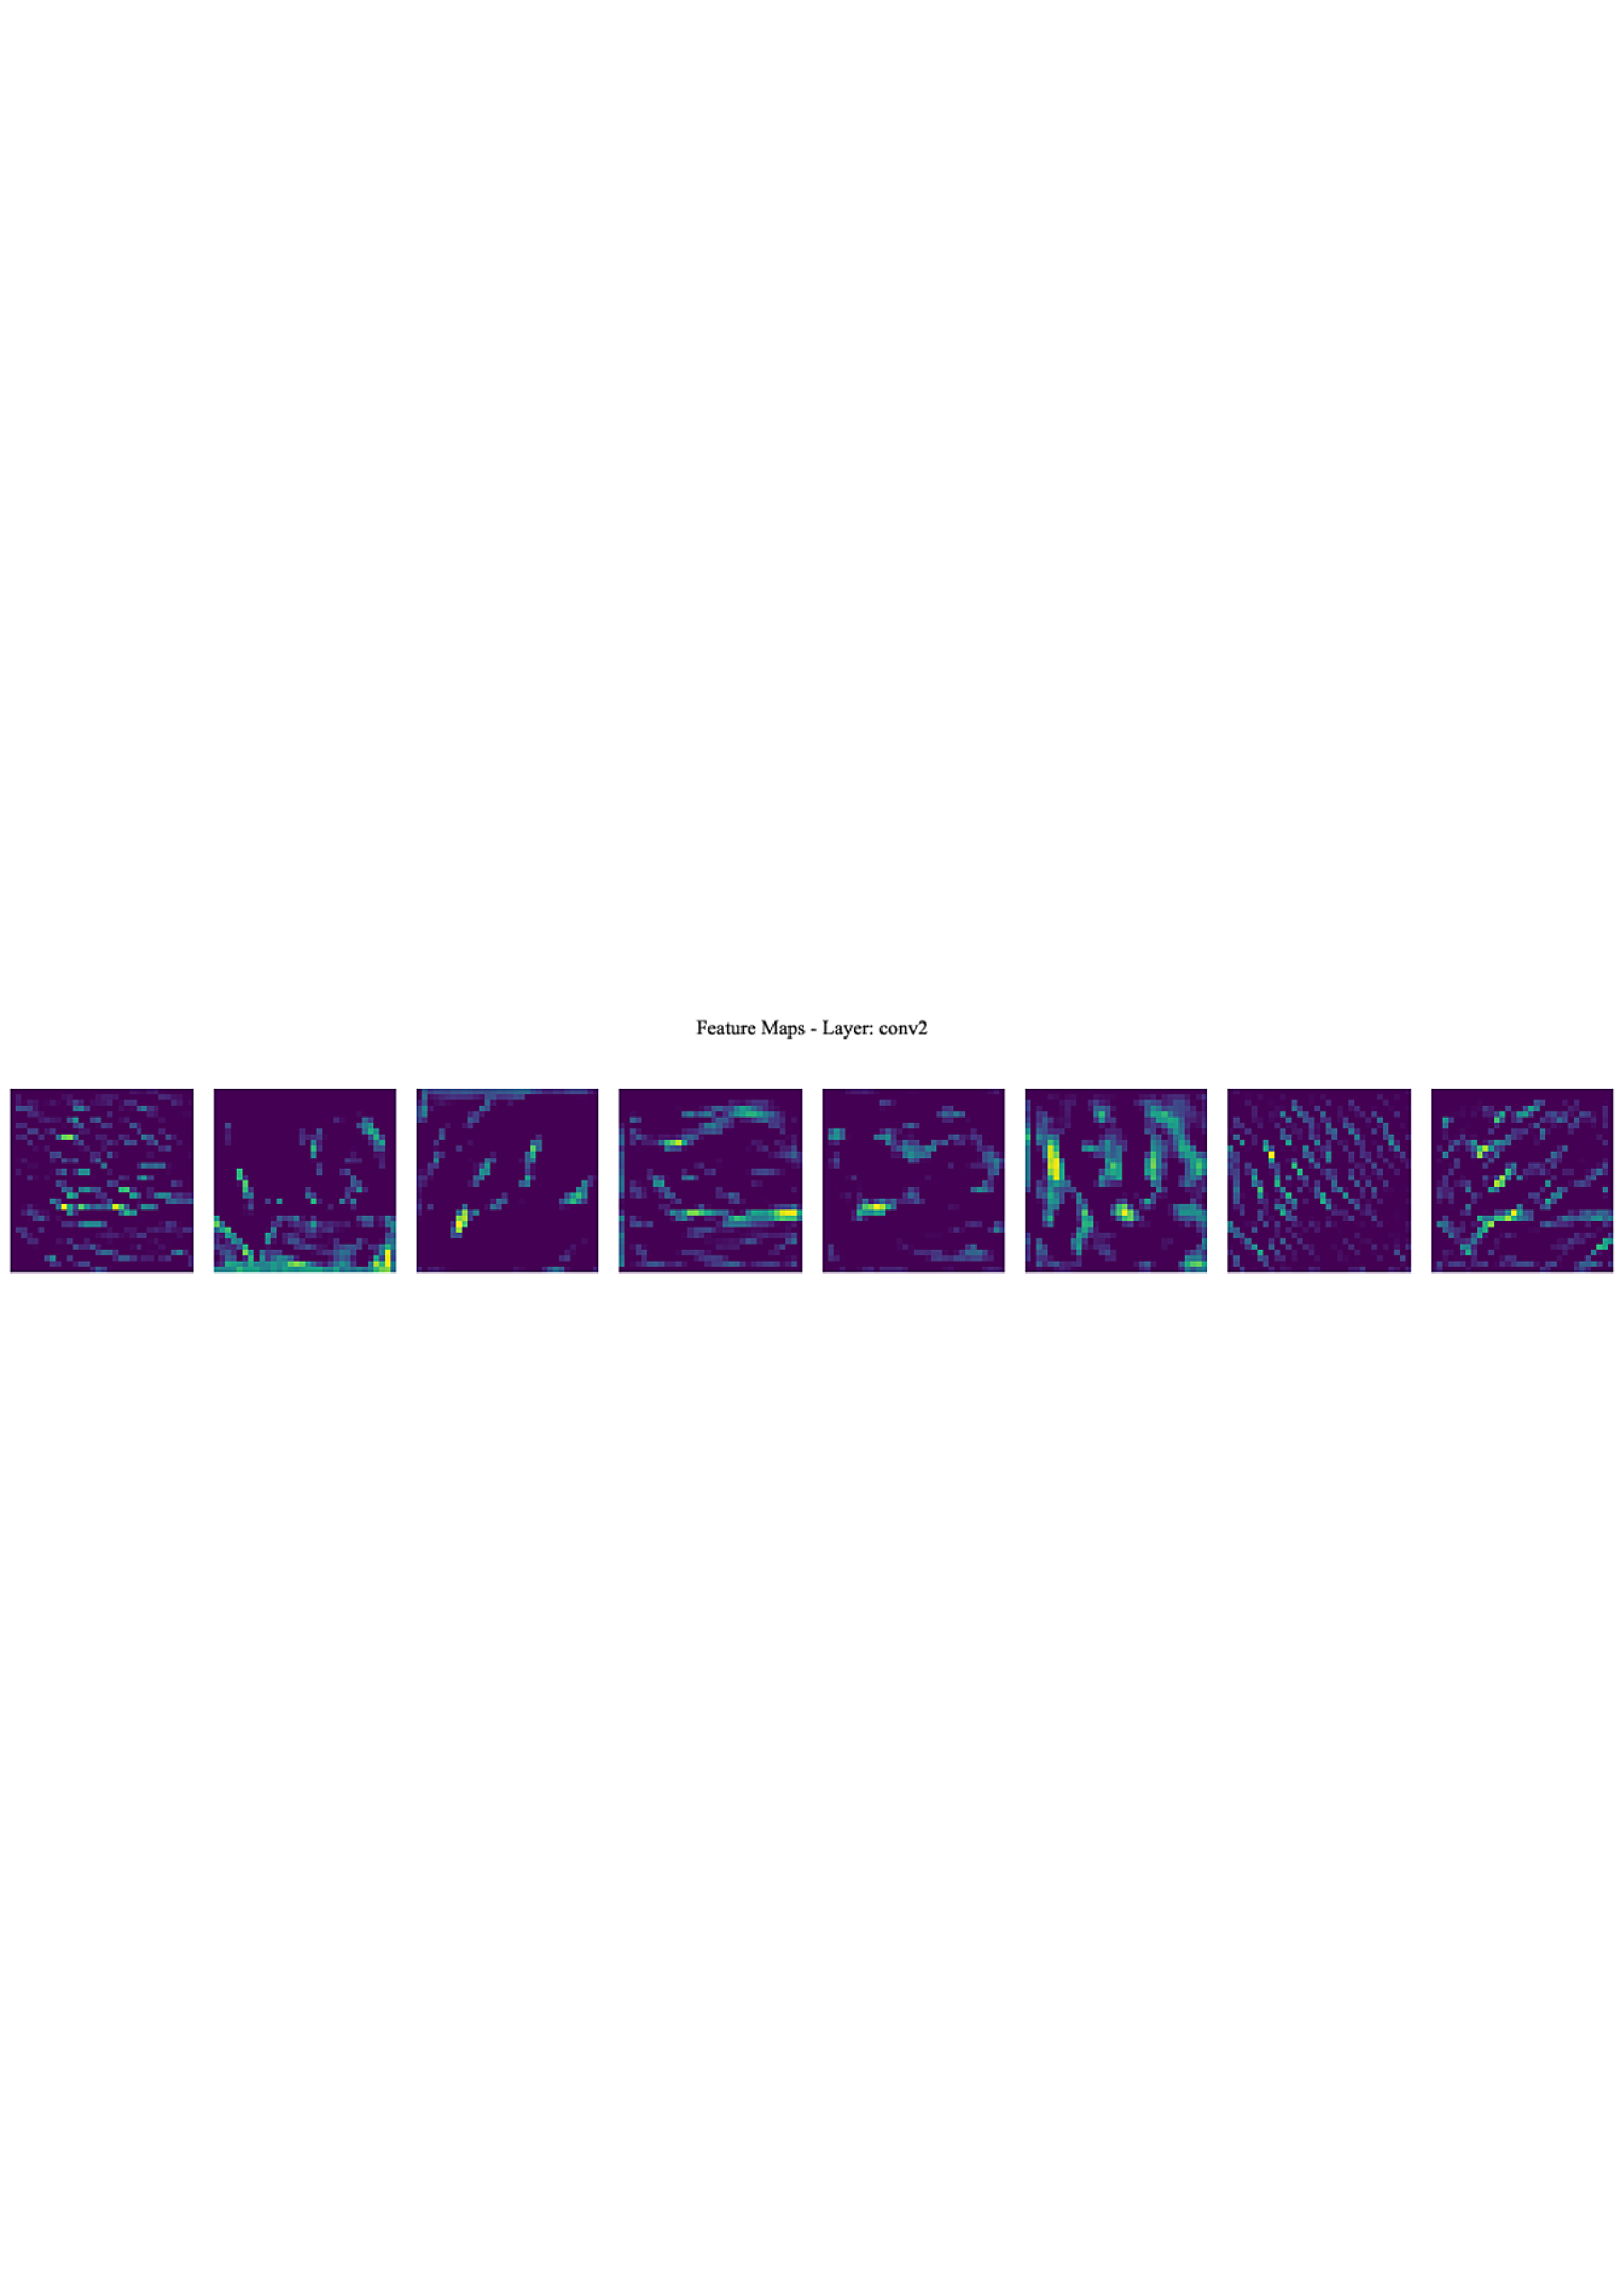
\includegraphics[width=\textwidth]{feature_maps_conv2.pdf}
\caption{Feature Maps -- Layer conv2 (Main CNN)}
\end{figure}
\textbf{Inference:} The second layer's maps are already less literal than conv1's -- the object's raw outline is fading, replaced by thinner, more directional streaks, suggesting the network is starting to respond to specific textures and orientations rather than the whole shape.

\begin{figure}[H]
\centering
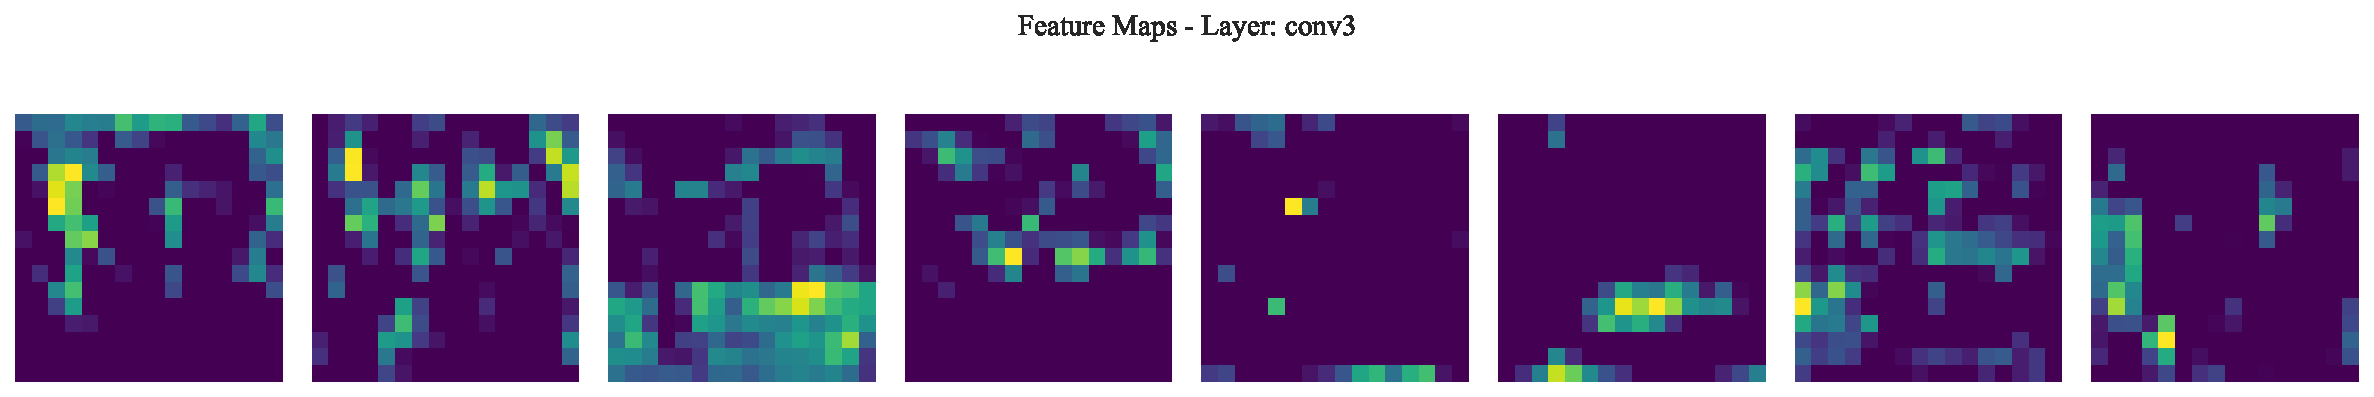
\includegraphics[width=\textwidth]{feature_maps_conv3.pdf}
\caption{Feature Maps -- Layer conv3 (Main CNN)}
\end{figure}
\textbf{Inference:} By the third layer, the feature maps are noticeably more abstract, and the spatial resolution has halved (32$\times$32 $\to$ 16$\times$16) from the first pooling step -- the network is combining low-level edges into more complex, part-based patterns.

\begin{figure}[H]
\centering
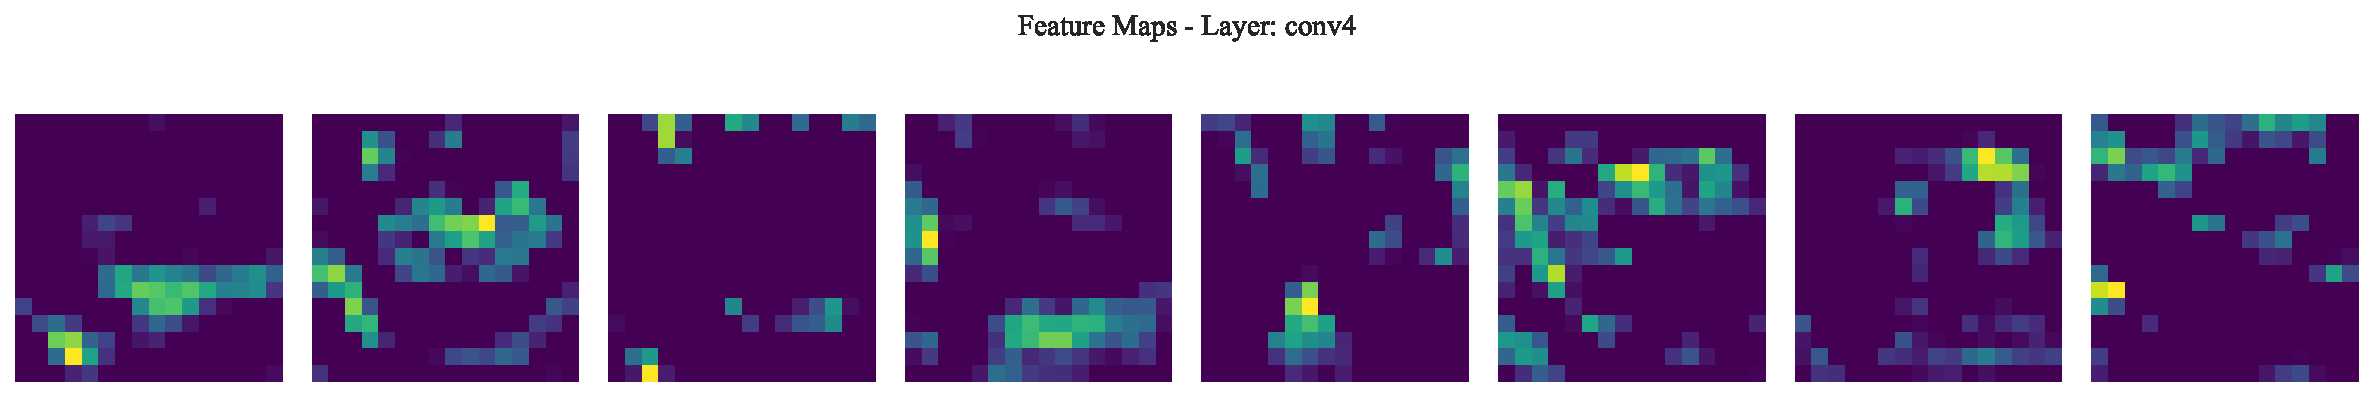
\includegraphics[width=\textwidth]{feature_maps_conv4.pdf}
\caption{Feature Maps -- Layer conv4 (Main CNN)}
\end{figure}
\textbf{Inference:} conv4 continues the same trend as conv3, but sparser -- fewer pixels fire strongly, and the ones that do trace out specific curved or angular sub-structures rather than broad regions.

\begin{figure}[H]
\centering
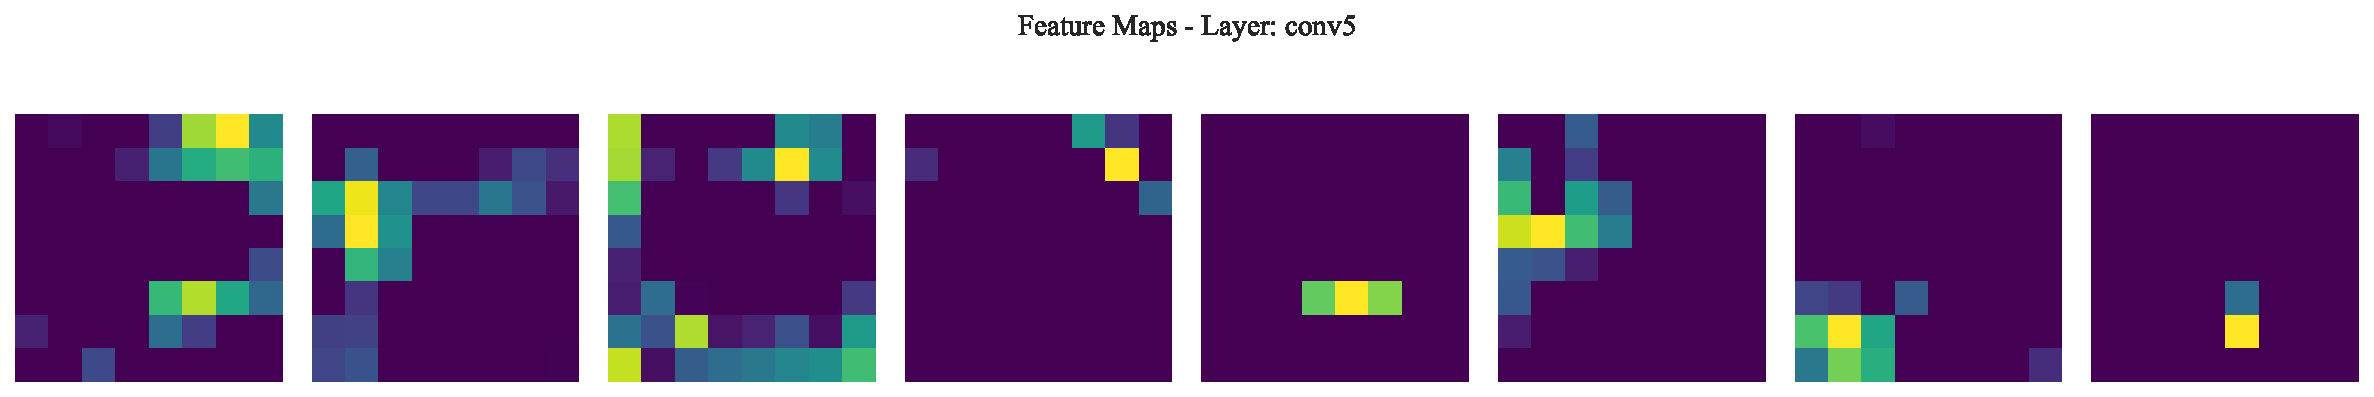
\includegraphics[width=\textwidth]{feature_maps_conv5.pdf}
\caption{Feature Maps -- Layer conv5 (Main CNN)}
\end{figure}
\textbf{Inference:} The deepest layer's maps are sparse and highly abstract, with only a handful of filters firing strongly -- the hierarchical feature learning CNNs are known for: early layers detect generic patterns, deep layers detect class-specific, high-level concepts.

\begin{figure}[H]
\centering
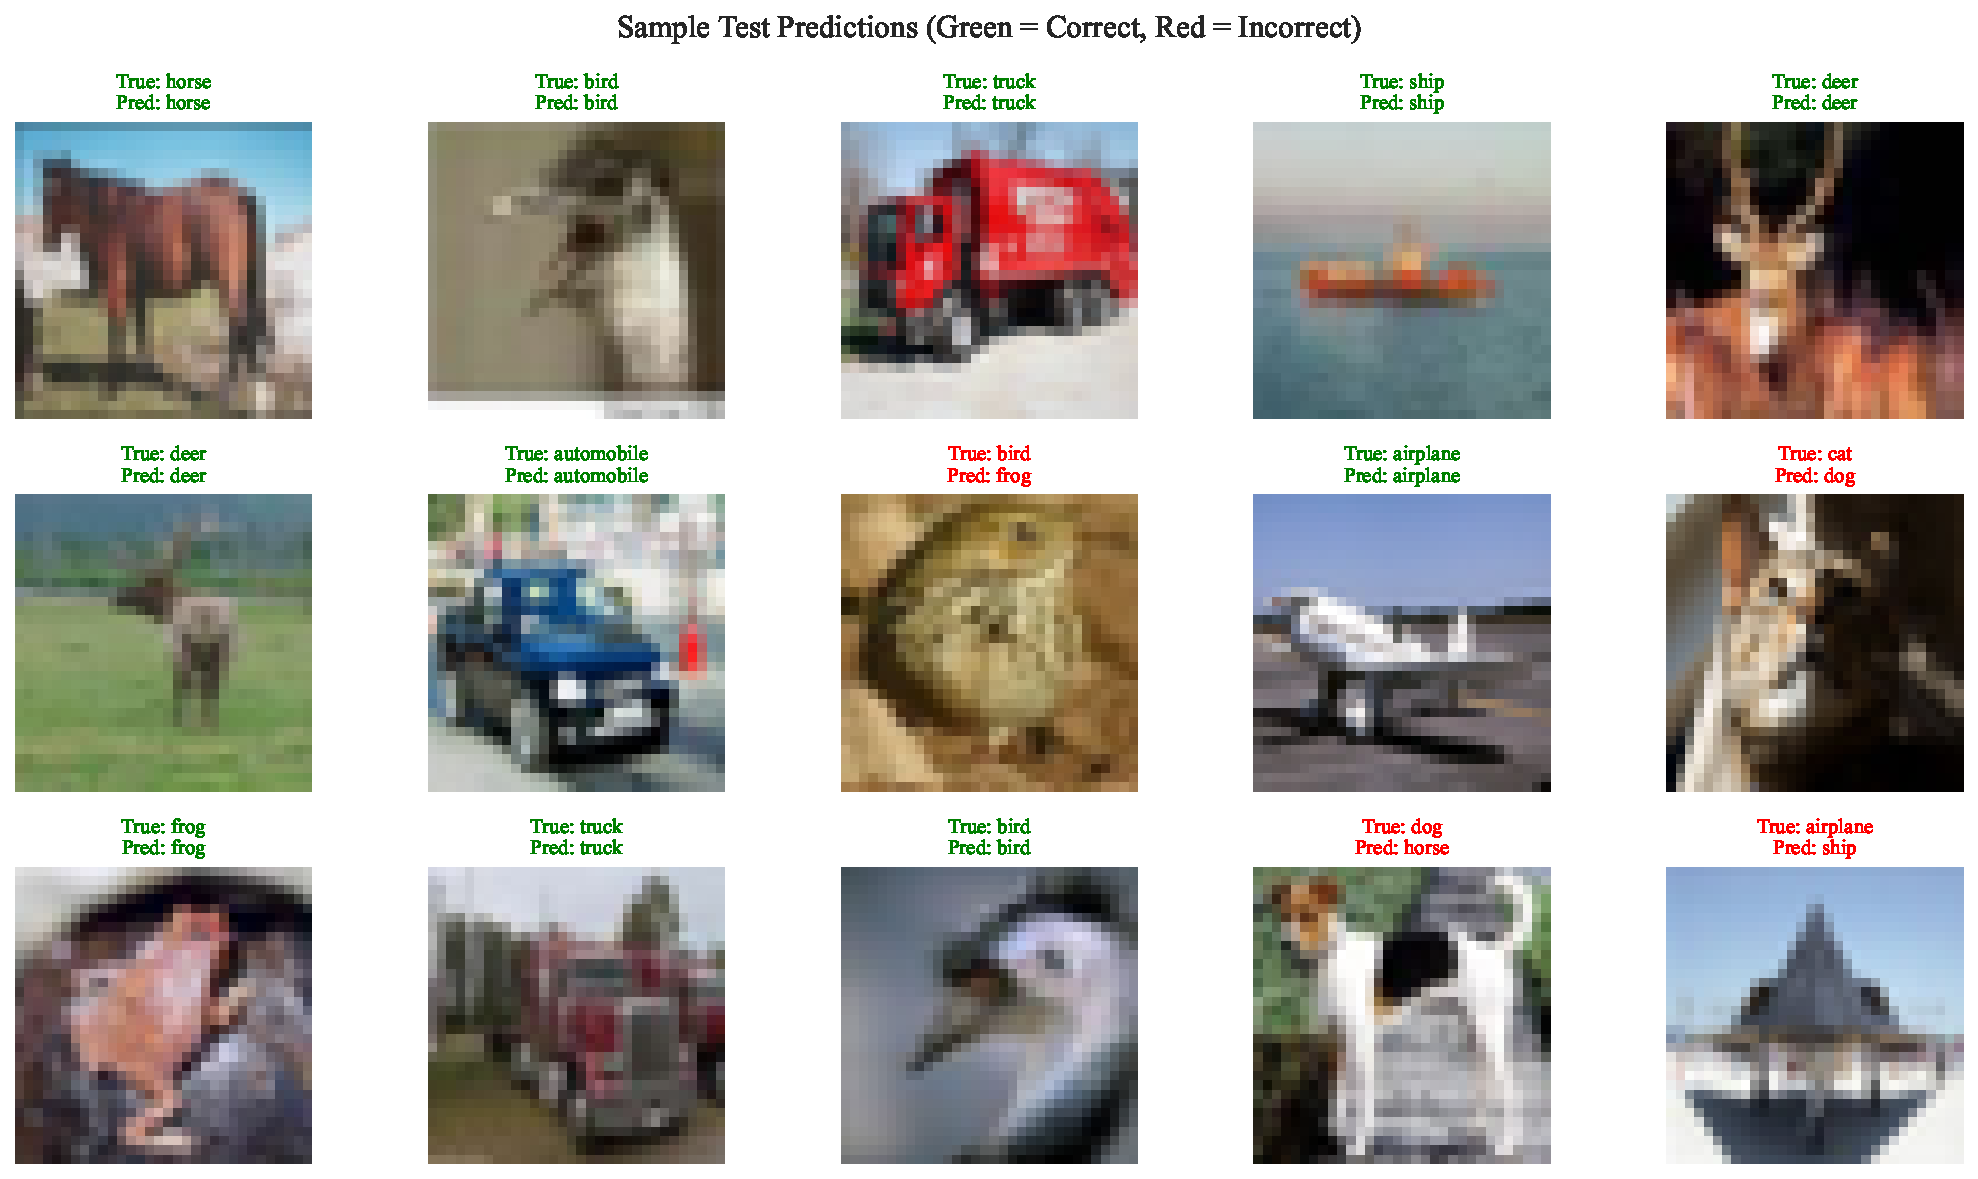
\includegraphics[width=0.9\textwidth]{sample_predictions.pdf}
\caption{Sample Test Predictions (Green = Correct, Red = Incorrect, Main CNN)}
\end{figure}
\textbf{Inference:} Correct predictions dominate the sample, and the visible mistakes cluster in exactly the classes the classification report already flagged as weaker -- the qualitative examples and the quantitative metrics tell the same story.

\begin{figure}[H]
\centering
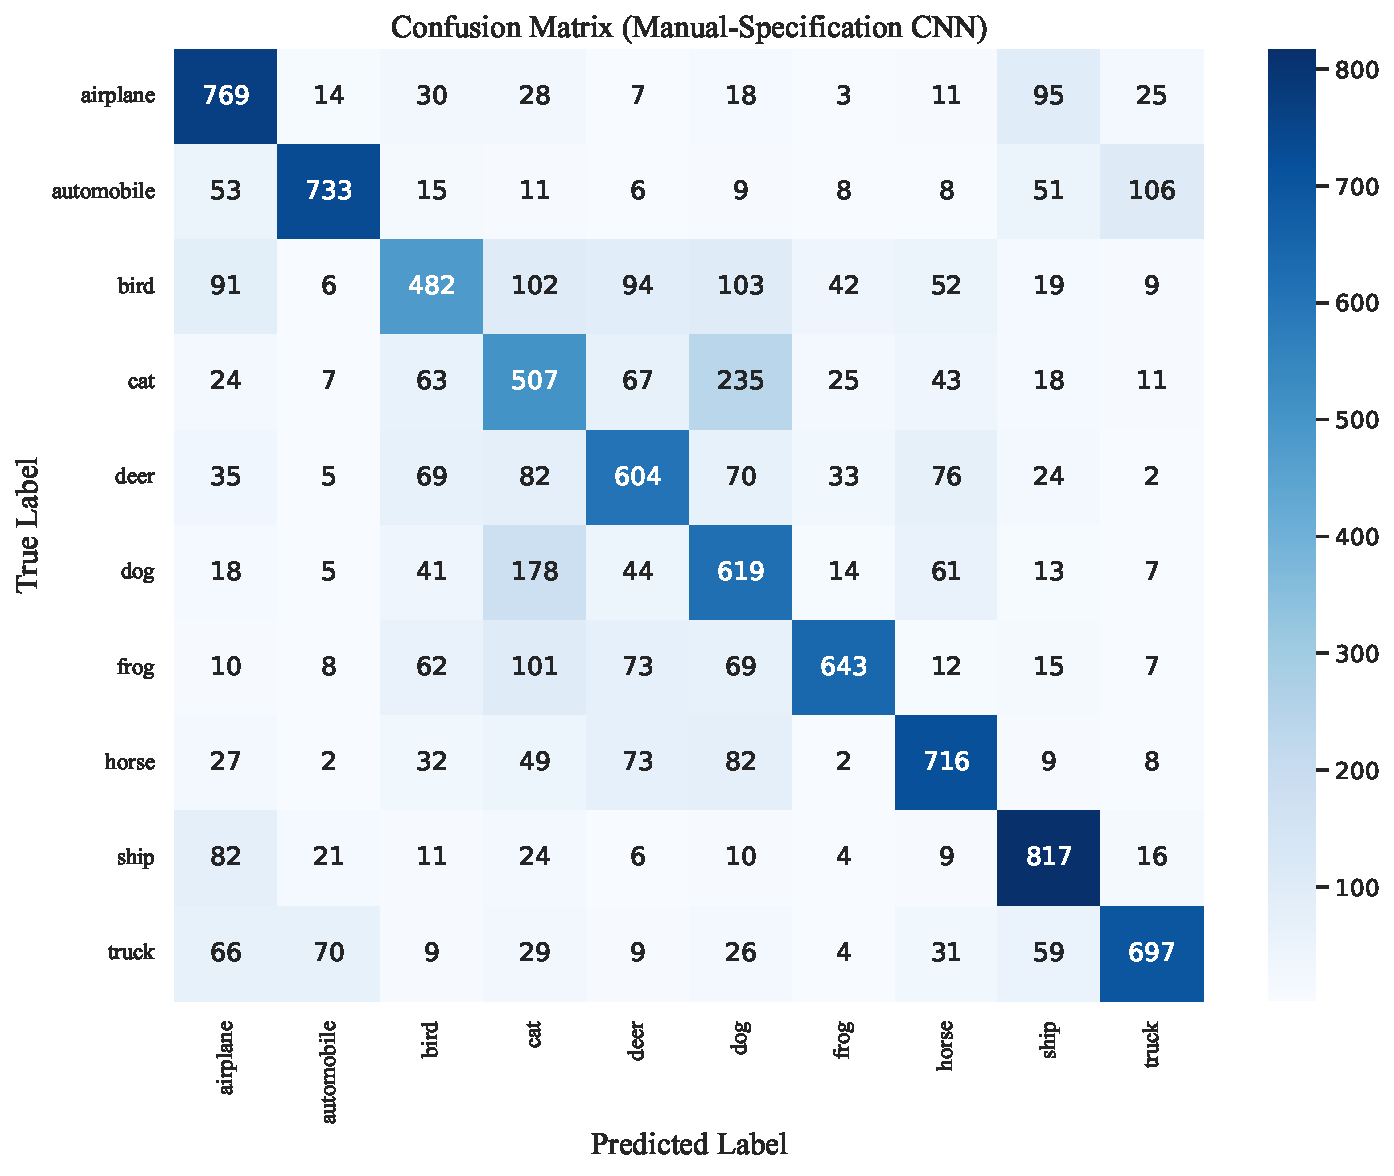
\includegraphics[width=0.6\textwidth]{confusion_matrix_manual_spec.pdf}
\caption{Confusion Matrix on the Test Set (Manual-Specification CNN, Task 6)}
\end{figure}
\textbf{Inference:} The diagonal is much weaker here than in the main CNN's confusion matrix, matching the 17-point accuracy gap between the two models -- cat and bird in particular show heavy confusion with several other classes, not just each other, reflecting this simpler model's lower overall capacity.

\begin{figure}[H]
\centering
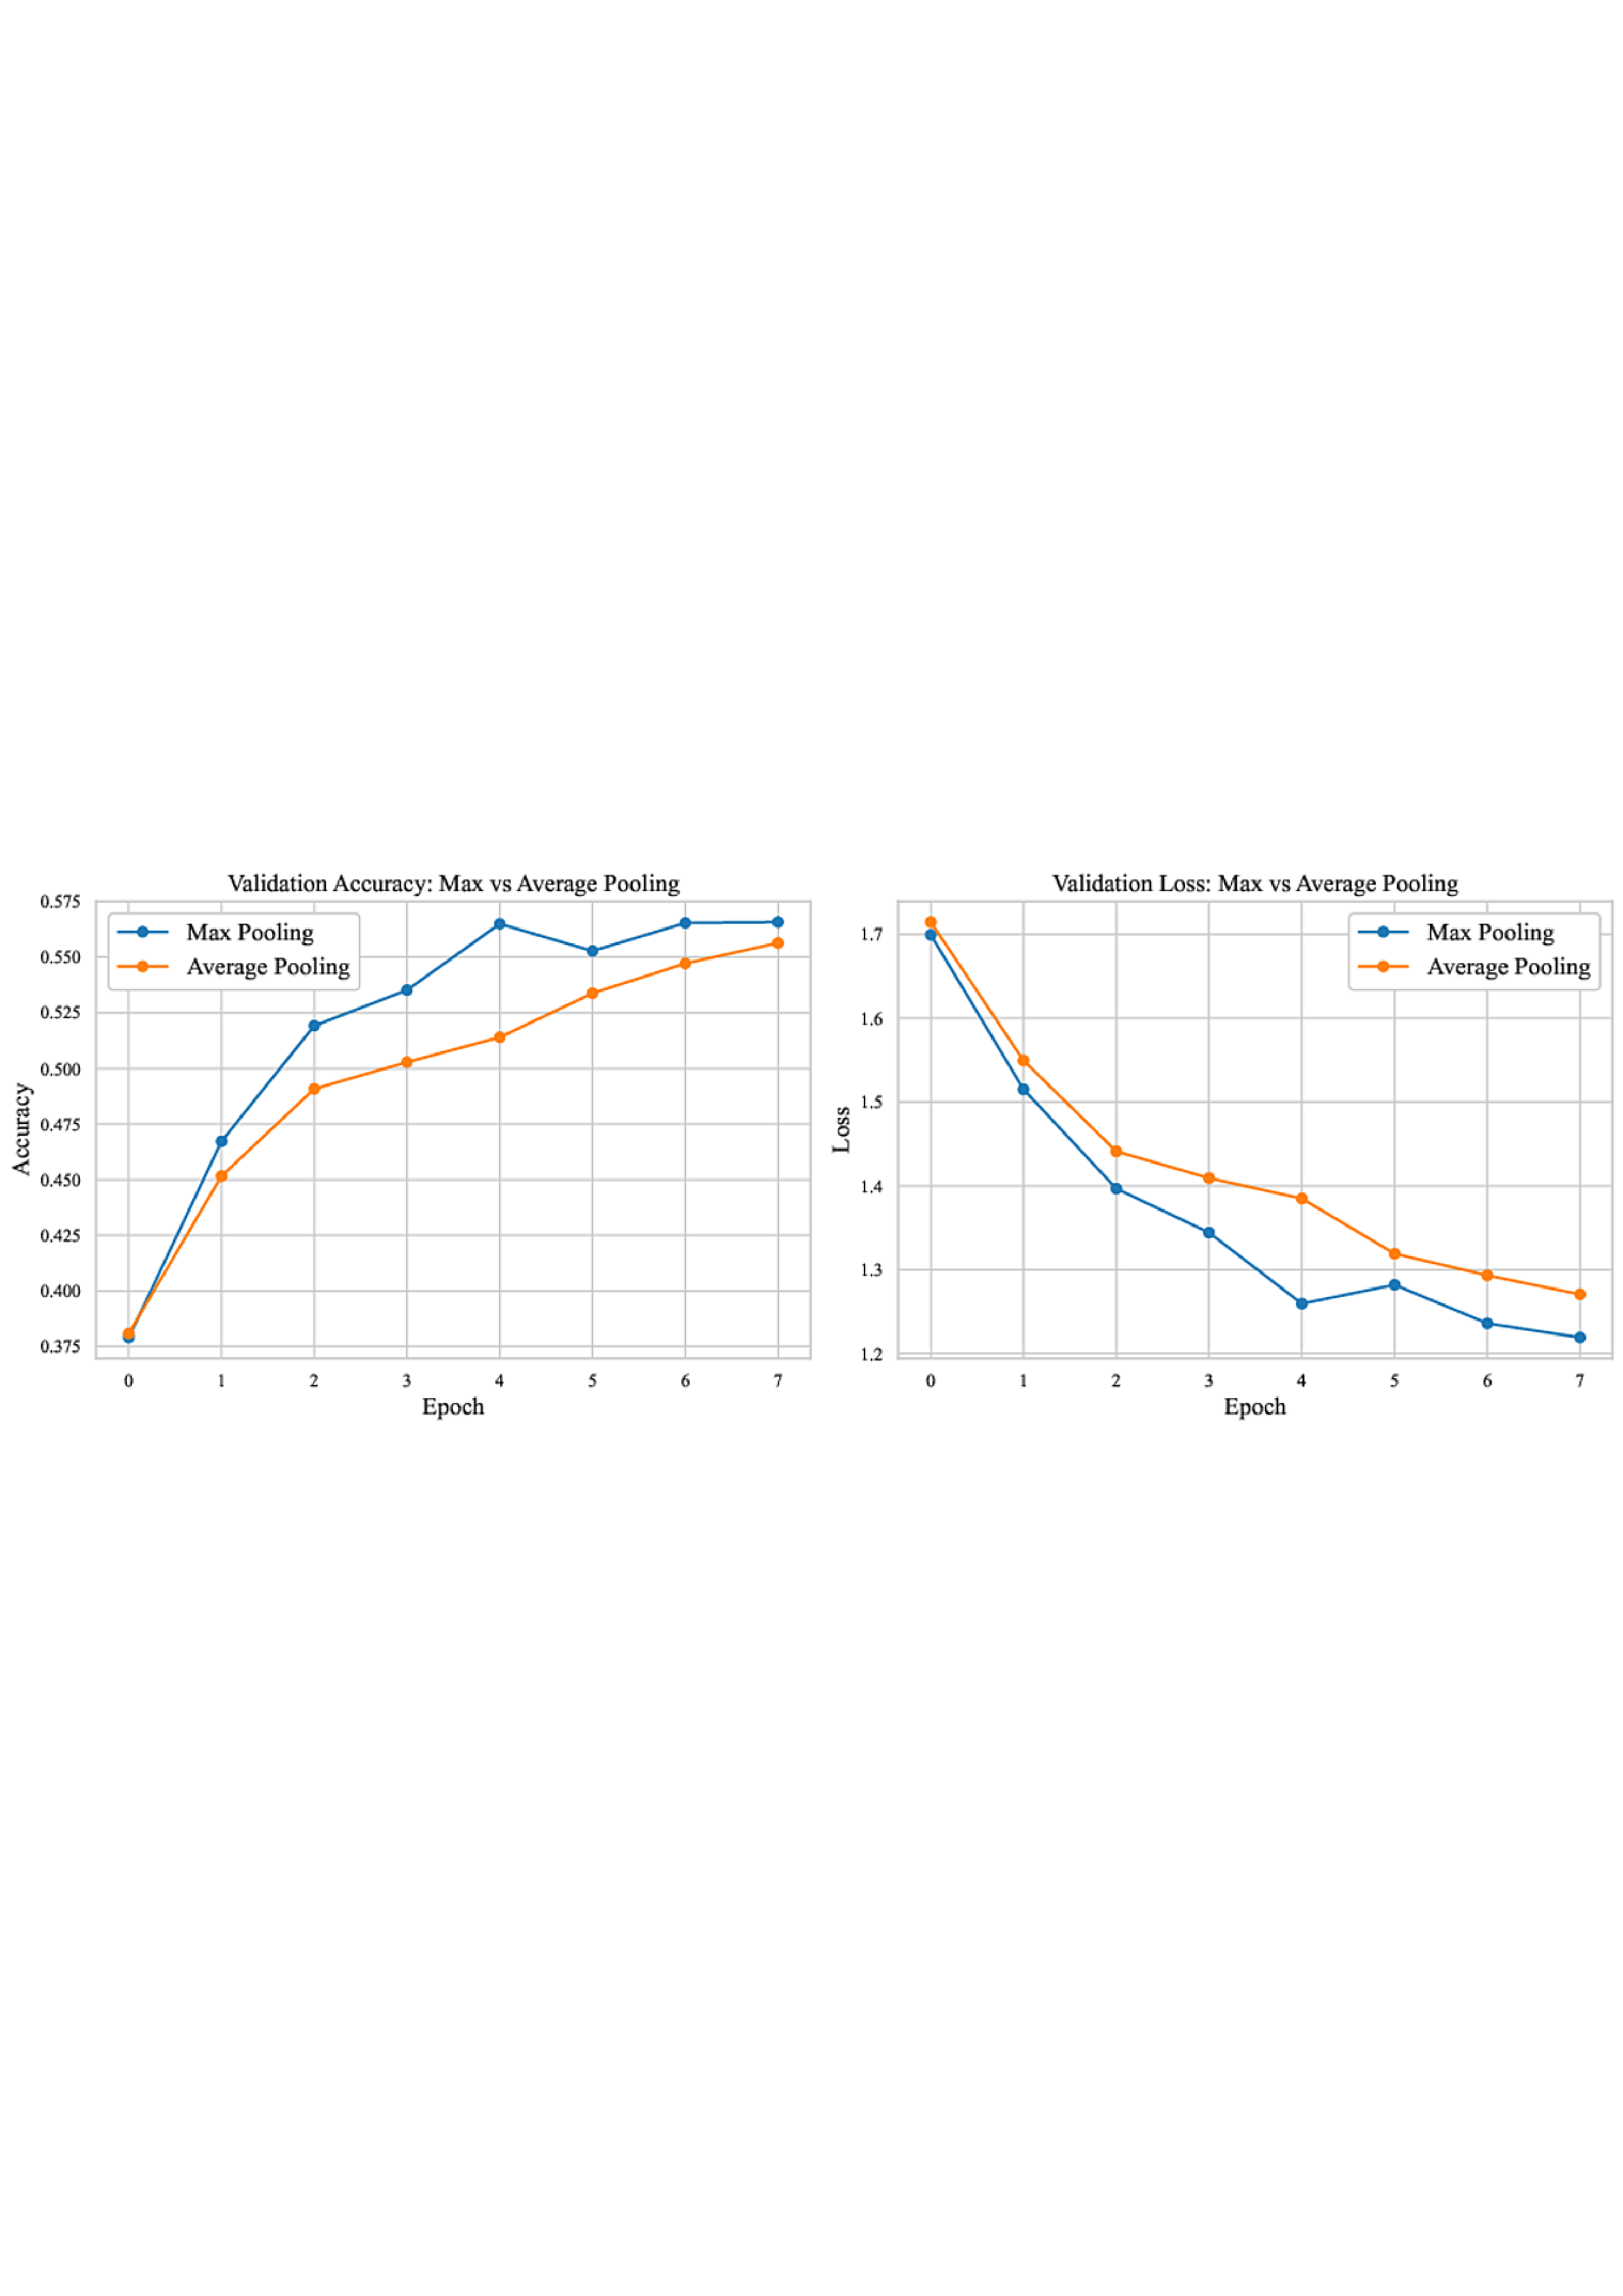
\includegraphics[width=0.9\textwidth]{pooling_comparison.pdf}
\caption{Validation Accuracy and Loss: Max vs. Average Pooling}
\end{figure}
\textbf{Inference:} The Max Pooling curve sits consistently at or above the Average Pooling curve across all 8 epochs, matching the final test accuracy gap (55.67\% vs. 54.32\%) reported in Section 10.6.

\begin{figure}[H]
\centering
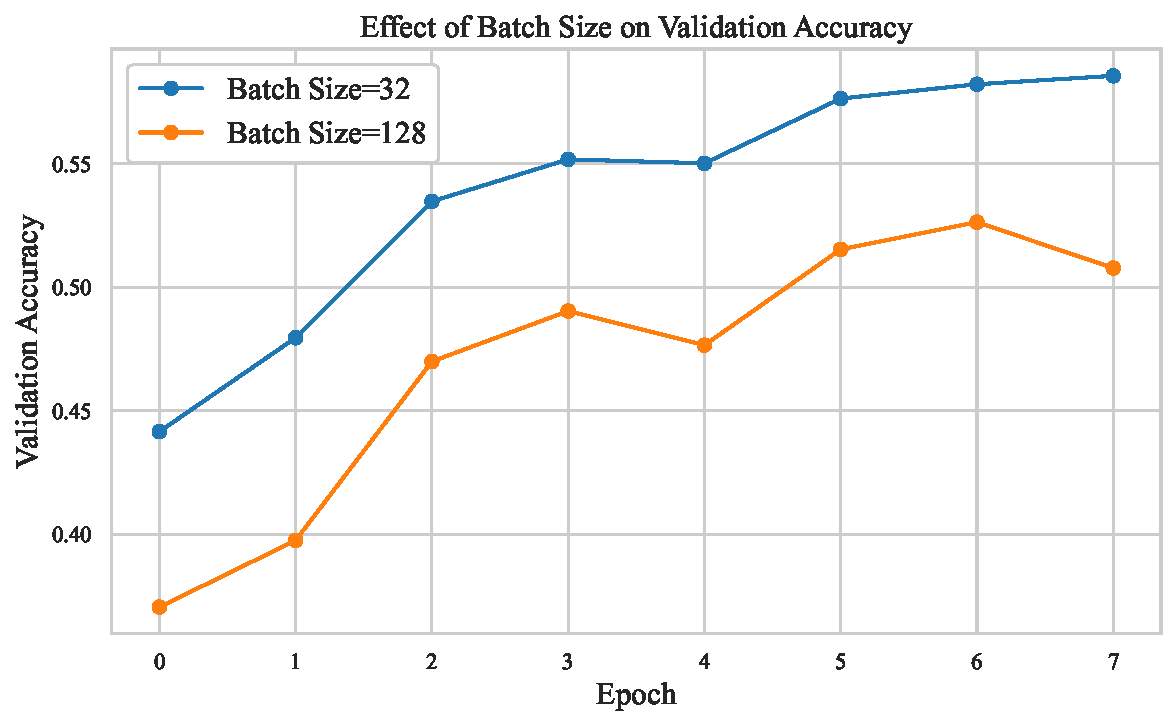
\includegraphics[width=0.6\textwidth]{batch_size_comparison.pdf}
\caption{Effect of Batch Size on Validation Accuracy}
\end{figure}
\textbf{Inference:} Batch size 32 (58.55\% test accuracy) clearly outperforms batch size 128 (51.45\%) under these matched short-training conditions -- more frequent, noisier weight updates appear to help this model more than the smoother, less frequent updates of the larger batch, at least within this many epochs.

\begin{figure}[H]
\centering
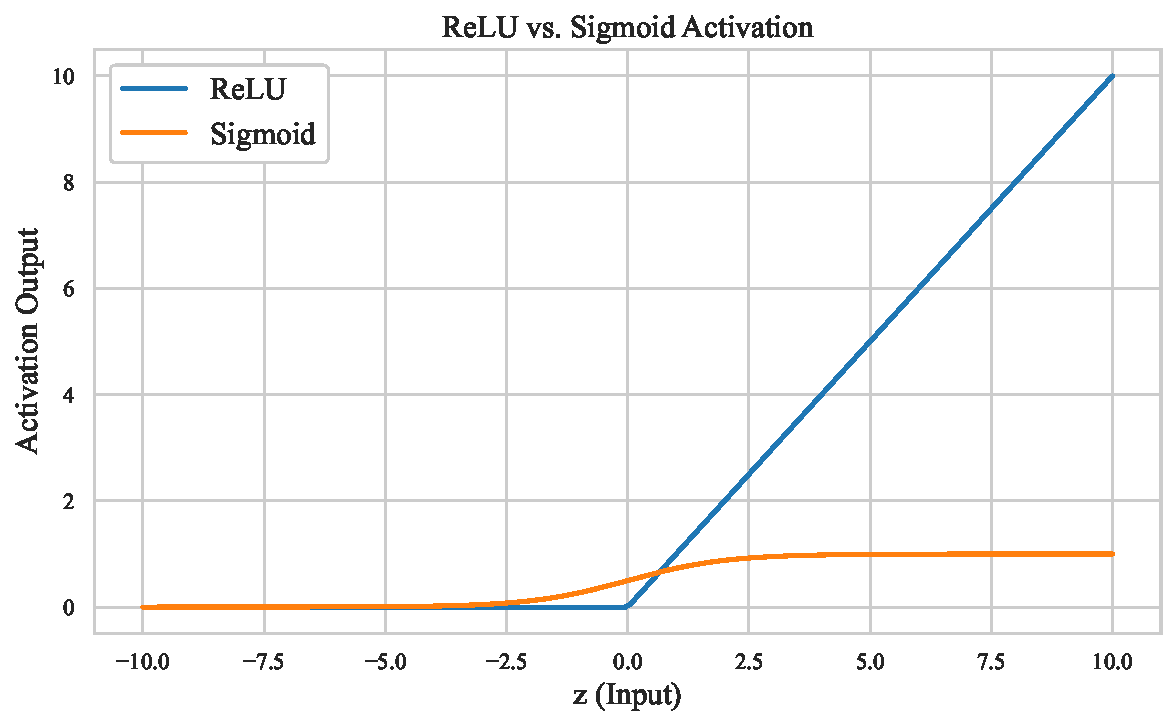
\includegraphics[width=0.7\textwidth]{relu_vs_sigmoid.pdf}
\caption{ReLU vs. Sigmoid Activation Functions}
\end{figure}
\textbf{Inference:} ReLU stays at zero for any negative input and passes positive values straight through, avoiding the vanishing-gradient problem that Sigmoid suffers from once its input moves far from zero -- exactly why every hidden layer in both CNNs in this notebook uses ReLU rather than Sigmoid.

%----------------------------------------------------------

\section*{13. Additional Exercises}

\textbf{1. Output size for a $64\times64$ image, $5\times5$ kernel, stride 2, padding 2.}
\[
\frac{64-5+2(2)}{2}+1 = \frac{63}{2}+1 = 32
\]
A $64\times64$ input with a $5\times5$ kernel, stride 2, padding 2 produces a $32\times32$ output feature map.

\textbf{2. Trainable parameters for 64 filters of size $3\times3$, RGB input.}
\[
(3\times3\times3+1)\times64 = 28\times64 = 1{,}792
\]

\textbf{3. Compare ReLU and Sigmoid activation functions.}
See Figure 19 (Section 12) and its inference above -- ReLU is cheap to compute and avoids vanishing gradients for active neurons, making it the standard choice for hidden layers; Sigmoid squashes outputs into $(0,1)$ but saturates for large-magnitude inputs, which is why it's mainly reserved for binary classification output layers rather than hidden layers in deep networks.

\textbf{4. Replace Max Pooling with Average Pooling and compare the results.}
Already covered in full in Section 10.6 and Figure 18 (Section 12) -- Max Pooling reached 55.67\% test accuracy versus Average Pooling's 54.32\%, with identical output shapes for both.

\textbf{5. Increase filters from 16 to 64 and analyze the effect on accuracy and computation time.}

\begin{table}[H]
\centering
\caption{Effect of Filter Count on Accuracy, Training Time, and Parameters}
\begin{tabular}{lccc}
\toprule
Filters (first conv layer) & Test Accuracy & Training Time & Parameters \\
\midrule
16 & 0.5401 & 11.9s & 25,578 \\
64 & 0.5929 & 15.0s & 157,578 \\
\bottomrule
\end{tabular}
\end{table}

Quadrupling the filter count (16 $\to$ 64) improved test accuracy by about 5.3 points, but at a real cost: parameters grew more than 6-fold (25,578 $\to$ 157,578) and training time increased by about 26\% (11.9s $\to$ 15.0s) for the same 8 epochs. More filters give the network a richer set of feature detectors, but that richness isn't free -- whether the accuracy gain justifies the extra time and memory depends entirely on the computational budget available.

%----------------------------------------------------------

\section*{14. Discussion}

\textbf{1. Why is convolution preferred over fully connected layers for images?}\\
Convolution uses a small set of shared weights (a kernel) that slides across the whole image, so it needs far fewer parameters than a fully connected layer would to look at every pixel independently, and it naturally captures local spatial patterns like edges and textures regardless of where they appear in the image.

\textbf{2. How does stride affect the feature map size?}\\
A larger stride moves the kernel by more pixels at each step, directly shrinking the output feature map -- as shown numerically in Section 10.5, stride 2 roughly halves the output size compared to stride 1 ($30\times30 \to 15\times15$).

\textbf{3. What is the role of padding?}\\
Padding adds extra pixels (usually zeros) around the input's border before convolution. `Same' padding keeps the output the same spatial size as the input, essential for building deep networks without the feature map shrinking to nothing after a few layers; `valid' padding uses no extra pixels and lets the output shrink naturally, as shown in Section 10.5.

\textbf{4. Why is pooling used?}\\
Pooling reduces the spatial size of feature maps, cutting computation and parameter count in later layers, while making the network somewhat robust to small shifts or distortions in where a feature appears.

\textbf{5. How do feature maps represent image characteristics?}\\
Each feature map is the response of one learned filter across the whole image -- high activation values mark where that pattern was detected. Early-layer feature maps (Section 11, conv1) look close to the original image since they detect simple edges; deeper-layer feature maps (Section 12, conv2-conv5) become progressively more abstract, as directly observed across this experiment.

\textbf{6. Why do CNNs require fewer parameters than MLPs?}\\
A fully connected layer needs a separate weight for every input-output pixel pair, which explodes for anything but tiny images. A convolutional layer instead uses one small kernel shared across every spatial position, so its parameter count depends only on kernel size and filter count -- not on the image's height and width at all, as demonstrated by the 60,362-parameter Task 6 model handling the same $32\times32\times3$ images as the 668,842-parameter main CNN.

%----------------------------------------------------------

\section*{15. Conclusion}

\begin{itemize}[leftmargin=*]
\item Built and trained two CNNs on CIFAR-10: a manual-specification model (Task 6, 60,362 parameters, 65.87\% test accuracy) and a larger, regularized CNN (668,842 parameters, 82.57\% test accuracy) -- directly demonstrating the accuracy cost of skipping batch normalization, dropout, and a deeper architecture.
\item Verified the convolution output-size formula numerically across kernel size, stride, and padding (Sections 10.4-10.5), matching hand-calculated values exactly.
\item Visualized feature maps across all five convolutional layers, observing the shift from edge-like, image-resembling activations in conv1 to sparse, abstract activations in conv5.
\item Compared Max Pooling and Average Pooling on both output size (identical) and accuracy (Max Pooling ahead by 1.4 points).
\item Directly observed the manual-specification model overfitting -- validation loss rising while training loss kept falling -- illustrating why the main CNN's regularization techniques exist.
\item Completed all five additional exercises, including a real accuracy/time/parameter trade-off measurement for increasing filter count from 16 to 64.
\end{itemize}

%----------------------------------------------------------

\section*{16. References}

\begin{enumerate}
\item I. Goodfellow, Y. Bengio and A. Courville, \emph{Deep Learning}, MIT Press, 2016.
\item C. M. Bishop, \emph{Pattern Recognition and Machine Learning}, Springer, 2006.
\item S. Haykin, \emph{Neural Networks and Learning Machines}, Pearson, 2009.
\item TensorFlow Documentation: \url{https://www.tensorflow.org}
\item CIFAR-10 Dataset Documentation -- University of Toronto.
\end{enumerate}

\end{document}
